We have implemented our approach in a prototype and compared it to three types of approaches 
(i) \deeppoly{}~\cite{singh2019abstract} and its refinements \kpoly{}~\cite{singh2019beyond}, \deepsrgr{}~\cite{yang2021improving}, 
(ii) other cegar based approaches, and 
%The approaches  \texttt{kPoly} and \texttt{deepSRGR} do the refinement on \deeppoly{}.
(iii) state-of-the-art tools \alphabeta~\cite{zhang2018efficient,wang2021beta,xu2020fast,zhang2022branch,tjeng2017evaluating}, 
\ovaltool~\cite{bunel2018unified,bunel2020branch,bunel2020lagrangian,de2021scaling,de2021scaling,de2021scaling2,de2021improved}, 
and \marabou~\cite{katz2019marabou}. 
Our tool is built upon \deeppoly{}, so we compare it with \deeppoly{} to establish a baseline. 
Furthermore, we compare our tool's performance with that of \kpoly{} and \deepsrgr{}, 
which are other refinement tools based on \deeppoly{}. 
We find that our tool performs well in comparison to these DeepPoly-based refinement tools.
As our tool is based on counterexample-guided refinement (CEGAR), we also compare it with other CEGAR-based tools. 
We also compare our tool with the latest version of \alphabeta{}, and 2021 version of \ovaltool{} and \marabou{}. 
Our results show that our tool is capable of solving unique benchmarks 
that are beyond the reach of current state-of-the-art tools.
Furthermore, we conducted a comparison of performance across different epsilon values for all the tools employed. 
We extended this analysis to focus specifically on adversarially trained networks and observed a significant improvement 
in performance. Moreover, we conducted a detailed comparison with \alphabeta{}, 
utilizing the same preprocessing steps employed by the \alphabeta{} tool.

The tools \alphabeta{} and \ovaltool{} use a set/portfolio of different algorithms and optimizations.
The tool \alphabeta{} achieved the first rank persistantly in both International Verification of Neural Networks Competition(VNN-COMP'21) and VNN-COMP'22.
The tool \marabou{} achieved the 6th ranks in VNN-COMP'22.  
The tool~\alphabeta{}, \ovaltool{}, and \marabou{} also achieved the 1st, 3rd, and 5th rank, 
respectively\footnote{We could not compare with \textsc{VeriNet}, which is the 2nd and 3rd of VNNCOMP 2021 and VNNCOMP 2022 respectively, as we had difficulties with its external solver's (\textsc{Xpress}) license. We also
could not compare with MN-BaB since it required GPU to run.  
Also, since we are comparing with \deeppoly{} and \kpoly{}, and \textsc{ERAN} uses these techniques internally, we skipped a direct comparison with \textsc{ERAN}, which achieved 4th rank in VNN-COMP'21.}, 
in VNN-COMP'21. We use the same configuration to run \alphabeta{} and \ovaltool{}, which these tools
used in VNN-COMP for mnist benchmarks.   

% We have implemented our approach in a prototype. We have presented out experiments in two subcategories. 
% In first category we compared our tool with most related state of the art tools. We created three types of approaches in this category, 
% (i) \deeppoly{}~\cite{singh2019abstract} and its refinements \kpoly{}~\cite{singh2019beyond}, \deepsrgr{}~\cite{yang2021improving}, 
% (ii) other cegar based approaches, and 
% %The approaches  \texttt{kPoly} and \texttt{deepSRGR} do the refinement on \deeppoly{}.
% (iii) state-of-the-art tools \alphabeta~\cite{zhang2018efficient,wang2021beta,xu2020fast,zhang2022branch,tjeng2017evaluating}, 
% \ovaltool~\cite{bunel2018unified,bunel2020branch,bunel2020lagrangian,de2021scaling,de2021scaling,de2021scaling2,de2021improved}, 
% and \marabou~\cite{katz2019marabou}. 
% Our tool is built upon \deeppoly{}, so we compare it with \deeppoly{} to establish a baseline. 
% Furthermore, we compare our tool's performance with that of \kpoly{} and \deepsrgr{}, 
% which are other refinement tools based on \deeppoly{}. 
% We find that our tool performs well in comparison to these DeepPoly-based refinement tools.
% As our tool is based on counterexample-guided refinement (CEGAR), we also compare it with other CEGAR-based tools. 
% We also compare our tool with \alphabeta{}, \ovaltool{}, and \marabou{}. 
% Our results show that our tool is capable of solving unique benchmarks 
% that are beyond the reach of current state-of-the-art tools.

% In second category we did the detailed comparison with \alphabeta{}, which is the 1st ranker in both 
% International Verification of Neural Networks Competition(VNN-COMP'21) and VNN-COMP'22. 
% The tools \alphabeta{} and \ovaltool{} use a set/portfolio of different algorithms and optimizations.
% The tool \marabou{} achieved the 6th ranks in VNN-COMP'22.  
% The tool~\alphabeta{}, \ovaltool{}, and \marabou{} also achieved the 1st, 3rd, and 5th rank, 
% respectively\footnote{We could not compare with \textsc{VeriNet}, which is the 2nd and 3rd of VNNCOMP 2021 and VNNCOMP 2022 respectively, as we had difficulties with its external solver's (\textsc{Xpress}) license. We also
% could not compare with MN-BaB since it required GPU to run.  
% Also, since we are comparing with \deeppoly{} and \kpoly{}, and \textsc{ERAN} uses these techniques internally, we skipped a direct comparison with \textsc{ERAN}, which achieved 4th rank in VNN-COMP'21.}, 
% in VNN-COMP'21.


\medskip

%We use the MNIST \cite{deng2012mnist} for our evaluation.    
%\subsection{Implementation}
\noindent{\bf Implementation.}
We have implemented our techniques in a tool, which we call \drefine{}, in \textsc{C++} programming language. Our approach relies on \deeppoly{}, so we also have implemented \deeppoly{} in \textsc{C++}. We are using a \textsc{C++} interface of the tool Gurobi~\cite{gurobioptimizer} to check the satisfiability as well as solve  \maxsat{} queries. %We have implemented our technique as a tool and call it \drefine{}.

%\subsection{Benchmarks}
\noindent{\bf Benchmarks.}
We use the MNIST~\cite{deng2012mnist} dataset to check the effectiveness of our tool and comparisons. We use 11 different fully connected feedforward neural networks with $\relu${} activation, as shown in Table~\ref{tb:nndetail}.
These benchmarks are taken from the \deeppoly{}'s paper~\cite{singh2019abstract}.  The input and output dimensions of each network are $784$ and $10$, respectively.  The authors of \deeppoly{} used projected gradient descent (PGD)~\cite{dong2018boosting}
and DiffAI~\cite{mirman2018differentiable} for adversarial training. Table \ref{tb:nndetail} contains the defended network i.e.
trained with adversarial training, as well as the undefended network. The last column of Table \ref{tb:nndetail} shows how the defended networks were trained.  

The predicate $P$ on the input layer is created using the input image $\boldsymbol{im}$ and user-defined 
parameter $\epsilon$.  We first normalize each pixel of $\boldsymbol{im}$ between $0$ and $1$, 
then create  $P = \Land_{i=1}^{|l_0|} im(i)-\epsilon \leq x_{0i}\leq im(i)+\epsilon$, such that the lower and upper 
bound of each pixel should not exceed $0$ and $1$, respectively. 
The predicate $Q$ on the output layer is created using the network's output.     
Suppose the predicted label of $\boldsymbol{im}$ on network $N$ is $y$, then $Q = \Land_{i=1}^{|l_k|} x_{ki} < y$, 
where $i \neq y$.  One query instance $\langle N,P,Q \rangle$ is created for one network, one image, and one epsilon 
value.  In our evaluation, we took $11$ different networks, 8 different epsilons, and 100 different images. 
The total number of instances is $8800$. However, there are $304$ instances for which the network's predicted label differs from the image's actual label. 
We avoided such instances and consider a total of $8496$ benchmark instances.    
% Whenever our tool found a counter-example on $\langle N,P,Q \rangle$, it denormalizes it into an image by rounding the 
% float values and checks for counter-example by executing $N$ on the denormalized image.
% If a counter-example is found then the tool reports it, otherwise, the tool reports unknown.


\begin{table}[t]
\centering
\scalebox{0.8}{
\begin{tabular}{c|c|c|c}
        \hline
        \textbf{Neural Network} & \textbf{\#hidden layers} & \textbf{\#activation units} & \textbf{Defensive training} \\
        \hline
        $3\times 50$ & 2 & 110 & None \\
        $3\times 100$ & 2 & 210 & None  \\
        $5\times 100$ & 4 & 410 & None  \\
        $6\times 100$ & 5 & 510 & DiffAI \\
        $9\times 100$ & 8 & 810 & None  \\
        $6\times 200$ & 5 & 1010 & None  \\
        $9\times 200$ & 8 & 1610 & None  \\
        $6\times 500$ & 6 & 3000 & None  \\
        $6\times 500$ & 6 & 3000 & PGD, $\epsilon = 0.1$ \\
        $6\times 500$ & 6 & 3000 & PGD, $\epsilon = 0.3$ \\
        $4\times 1024$ & 3 & 3072 & None  \\
        \hline
    \end{tabular}
    }
    \caption{Neural networks details}
    \label{tb:nndetail}
\end{table}
\begin{figure}[t]
    % \centering
    
\begin{tikzpicture}
    \begin{axis}[
        xlabel={Number of benchmarks},
        ylabel={log(time)},
        width=13cm,
        height=9cm,
        xmin=0, xmax=7000,
        ymin=0, ymax=25,
        xtick={0,1000,2000,3000,4000,5000,6000,7000},
        ytick={0,5,10,15,20,25},
        legend pos=south east,
        legend entries={drefine, deeppoly, deep\_SRGR, refinepoly, drefine\_verified, alpha\_beta, oval, cegar\_nn},
        ymajorgrids=true,
        xmajorgrids=true,
        grid style=dashed,
    ]
    \addplot[
        color=blue
    ] 
    table {fig/drefine_data.txt};
    
    \addplot[
        color=red
    ] 
    table {fig/deeppoly_data.txt};

    \addplot[
        color=orange
    ] 
    table {fig/deepsrgr_data.txt};

    \addplot[
        color=green
    ] 
    table {fig/refinepoly_data.txt};

    \addplot[
        color=violet
    ]
    table {fig/drefine_verified_data.txt};
    
    \addplot[
        color=purple
    ]
    table {fig/alpha_beta_data.txt};

    \addplot[
        color=brown
    ]
    table {fig/oval_data.txt};

    \addplot[
        color=gray
    ]
    table {fig/four_class_data.txt};

    \end{axis}

\end{tikzpicture}
    \caption{Cactus plot with most related techniques}
    \label{res:milp_with_milp}
\end{figure}


\subsection{Results}
We conducted the experiments on a machine with \textsc{64GB RAM, 2.20 GHz Intel(R) Xeon(R) CPU E5-2660 v2}
processor with CentOS Linux 7 operating system. 
To make a fair comparison between the tools, we provide only a single \textsc{CPU}, and $2000$ seconds timeout for each instance for each tool. 
We uses vanilla \deeppoly{}(\deeppoly{} without preprocessing in line 1 of algorithm~\ref{algo:main}) 
to generate kthe abstract constraints of benchmarks instances.
Figure~\ref{res:milp_with_milp} represents the cactus plot of (log of) time taken vs the number of benchmarks 
solved for the most related techniques. Table~\ref{tb:matrix} and \ref{tb:matrix1} represent a 
pairwise comparison of the number of 
instances that a tool could solve which another couldn't  
(more precisely, the $(i,j)$-entry of the table is the number of instances which could be verified 
by tool $i$ but not by tool $j$), and Figure~\ref{res:ep:milp_with_milp}, compares wrt epsilon, the robustness parameter.

% \subsubsection{Comparison with state of the arts:}

% In this category we uses vanilla \deeppoly{}(\deeppoly{} without preprocessing in line 1 of algorithm~\ref{algo:main})
% to generate kthe abstract constraints of benchmarks instances. 
% We make three types of comparisons as shown in (i) Figure~\ref{res:milp_with_milp}, which is a cactus plot of (log of) time taken vs the number of benchmarks solved for the most related techniques (ii) Table~\ref{tb:matrix}, which makes a pairwise comparison of the number of instances that a tool could solve which another couldn't  (more precisely, the $(i,j)$-entry of the table is the number of instances which could be verified by tool $i$ but not by tool $j$) and (iii) Figure~\ref{res:ep:milp_with_milp}, which compares wrt epsilon, the robustness parameter.
%represents the verified cases while the column represents the not verified cases, i.e.\kpoly{}'th row and \deeppoly{}'th column represent the  156 number of benchmarks instances which are solved by \kpoly{} and not solved by \deeppoly{}. 




\paragraph{Comparison with the most related techniques:}
In this subsection, we consider the techniques \deeppoly{}, \kpoly{}, and \deepsrgr{} to compare with ours. 
We consider \deeppoly{} because it is at the base of our technique, and the techniques \kpoly{} and \deepsrgr{} refine \deeppoly{} just as we do. These tools only report \verified{} instances, while our tool can report  \verified{} and counter-example. Hence, we compare these techniques with only \verified{}  instances of our technique in the line of \textsc{drefine\_verified} in cactus plot ~\ref{res:milp_with_milp}. 

Our technique outperforms the others in terms of the verified number of instances. One can also see that when they do verify, \deeppoly{} and \kpoly{} are often more efficient, which is not surprising, while our tool is more efficient than \deepsrgr{}. From Table~\ref{tb:matrix}, we also see  that our tool solves all the benchmark instances which are solved by these three techniques (and in fact around $\sim 700$ more), %\todo{check this number - was written 3700) for \deeppoly{} and \kpoly{} and $\sim 1000$ for \deepsrgr),
% \todo{afzal, check. this number was written 3700 and 1000-- its only 700 acc to table}
except $14$ instances where \kpoly{} succeeds and our tool times out.


% The approaches \deeppoly{}, \texttt{refinepoly}, and \texttt{deepSRGR} are incomplete and do not report the counter-example. 
% Our approach is a complete approach. We compare our approach's \texttt{verified} only instances with incomplete approaches. 
% Figure~\ref{res:milp_with_milp} shows the comparison with the help of the cactus plot. Our approach performs well 
% in terms of the verified number of instances as well as in terms of time in comparison to the above incomplete approaches. 
% We are also comparing with state of the arts to check the effectiveness of our approach globally.
% Table~\ref{tb:soacomparison} shows that our tool is verifying $180$ and $190$ benchmarks which $\alpha -\beta$-CROWN and 
% \texttt{oval} respectively are not able to verify. In addition to this, our tool verifies $172$ unique instances 
% that neither $\alpha -\beta$-CROWN nor \texttt{oval} is able to verify.  
% Despite it, $\alpha - \beta-$Crown and \texttt{oval} are verifying more benchmarks in comparison to our tool. 
% Although the total time taken by both state of the arts is higher than our tool as shown in figure~\ref{res:milp_with_milp}. 


% \begin{table}
%     \centering
%     \begin{tabular}{|c|c|c|c|}
%         \hline
%         -  & Not verified by oval & Not verified by $\alpha - \beta$-CROWN & Not verified by both \\
%         \hline
%         Verified by our tool & 190 & 180 & 172 \\
%         \hline
%     \end{tabular}
%     \caption{Comparison with $\alpha - \beta$-CROWN and Oval}
%     \label{tb:soacomparison}
% \end{table}





\paragraph{Comparison with cegar based techniques: }
\cegarnn{}~\cite{elboher2020abstraction} is a tool that also uses  counter example guided refinement. But the abstraction used is quite different from \deeppoly{}. This tool reduces the size of the network by merging similar neurons, such that they maintain the overapproximation and split back in the refinement process. We can conclude from Table~\ref{tb:matrix} that \cegarnn{} verified only  $18.88\%$, while our tool verified $61.42\%$ of the total number of benchmark instances. Although, in total \cegarnn{} solves significantly fewer benchmarks, it is pertinent to note that this technique solves many unique benchmark instances as can be inferred from Table~\ref{tb:matrix}. %Again this shows the orthogonal nature of this technique compared to the others.% the tool \texttt{cegar\_nn} is deployed completely different technique in comparison to others. 


\paragraph{Comparison with state-of-the-art solvers: }
The tools \alphabeta{} and \ovaltool{} use several algorithms that are highly optimized and use several techniques. 
The authors of \alphabeta{} implement the techniques~\cite{zhang2018efficient,wang2021beta,xu2020fast,zhang2022branch,tjeng2017evaluating}, 
and the authors of \ovaltool{} implement~\cite{bunel2018unified,bunel2020branch,bunel2020lagrangian,de2021scaling,de2021scaling,de2021scaling2,de2021improved}.
The authors of \marabou{} implement the technique~\cite{katz2019marabou}. 
Table~\ref{tb:matrix} shows that all three tools indeed solve about 1000 (out of 8496) more than 
we do\footnote{\alphabeta{} outperforms \marabou{} in VNN-COMP'22, while in our experiments \marabou{} performs better; potential reasons could be difference in benchmarks and that \alphabeta{} uses \textsc{GPU}, while \marabou{} uses \textsc{CPU} in VNN-COMP'22.}. 
However, we found around $180$ benchmarks instances where \alphabeta{} fails, and our tool works, 
and around $190$ benchmarks on which \ovaltool{} fails and our tool works. 
Also, around $655$ benchmarks where \marabou{} fails and our tool works; see Table~\ref{tb:matrix} for more details. 
In total, we are solving $59$ unique benchmarks where all three tools fail to solve. 
Thus we believe that these tools are truly orthogonal in their strengths and could potentially be combined. 
% We also note that in terms of total time, both tools take more time than our tool. 


% \definecolor{Gray}{gray}{0.6}
% \definecolor{LightRed}{rgb}{0.6,0,0}
% \definecolor{Lightgreen}{rgb}{0.88,1,1}

\newcolumntype{g}{>{\columncolor{red!20}}c}

% \begin{table}[t]
%   \scriptsize
%     \centering
%     \begin{tabular}{|c|c|c|c|c|c|c|c|g||c|}
%         \hline
%         \diagbox{\tiny Verified}{\tiny Not verified} & \tiny \textbf{\marabou} & \tiny \textbf{\cegarnn} & \tiny \textbf{\deeppoly} & \tiny \textbf{\kpoly} & \tiny \textbf{\deepsrgr} & \tiny \textbf{\alphabeta} & \tiny \textbf{\ovaltool} & \tiny \textbf{\drefine} & \tiny \textbf{\textsc{total}} \\
%         \hline
%         \tiny \textbf{\marabou} & \textbf{0} & 4741 & 2042 & 1892 & 2006 & 994 & 1005 &  1624 & 6292 \\
%         \hline
%         \tiny \textbf{\cegarnn} & 87 & \textbf{0} & 713 & 609 & 687 & 217 & 238 & 417 &  1638 \\ 
%         \hline
%         \tiny \textbf{\deeppoly} & 383 & 3708 & \textbf{0} & 0 & 0 & 63 & 66 & 0  & 4633 \\ 
%         \hline
%         \tiny \textbf{\kpoly} & 389 & 3760 & 156 & \textbf{0} & 114 & 63 & 66 & 14  & 4789  \\ 
%         \hline
%         \tiny \textbf{\deepsrgr} & 401 & 951 & 54 & 2 & \textbf{0} & 63 & 66 & 0  & 4687 \\ 
%         \hline
%         \tiny \textbf{\alphabeta} & 944 & 4821 & 1672 & 1516 & 1618 & \textbf{0} & 84 & 1095  & 6242 \\
%         \hline
%         \tiny \textbf{\ovaltool} & 902 & 4789 & 1622 & 1466 & 1568 & 31 & \textbf{0} & 1052 & 6189  \\
%         \hline
%         \rowcolor{green!20}
%         \tiny \textbf{\drefine} & 655 & 4106 & 694 & 552 & 640 & 180 & 190 & \textbf{0} & 5327 \\
%         \hline
%     \end{tabular}
%     \caption{Pairwise comparison of tools, e.g. entry on row \kpoly{} and column \deeppoly{} represents 156 benchmark instances on which \kpoly{} verified but \deeppoly{} fails. The green row highlights the number of solved benchmark instances by \drefine{} and not others while the red column is the opposite.}
%     \label{tb:matrix}
% \end{table}

\begin{table}[t]
  \scriptsize
    \centering
    \begin{tabular}{|c|c|c|c|c|c|c|c|g||c|}
        \hline
        \diagbox{\tiny Verified}{\tiny \mbox{}\hspace{-2mm}Unverified} & \tiny \textbf{\deeppoly} & \tiny \textbf{\kpoly} & \tiny \textbf{\deepsrgr} & \tiny \textbf{\cegarnn} & \tiny \textbf{\alphabeta} & \tiny \textbf{\ovaltool} & \tiny \textbf{\marabou} & \tiny \textbf{\drefine} & \tiny \textbf{\textsc{total}} \\
        \hline
        \tiny \textbf{\deeppoly} & \textbf{0} & 0 & 0 & 3708 & 63 & 66 & 383 &  0 & 4633 \\
        \hline
        \tiny \textbf{\kpoly} & 156 & \textbf{0} & 114 & 3760 & 63 & 66 & 389 & 14 &  4789 \\ 
        \hline
        \tiny \textbf{\deepsrgr} & 54 & 2 & \textbf{0} & 3736 & 63 & 66 & 401 & 0  & 4687 \\ 
        \hline
        \tiny \textbf{\cegarnn} & 713 & 609 & 687 & \textbf{0} & 217 & 238 & 87 & 417  & 1624  \\ 
        \hline
        \tiny \textbf{\alphabeta} & 1672 & 1516 & 1618 & 4821 & \textbf{0} & 84 & 944 & 1095  & 6242 \\ 
        \hline
        \tiny \textbf{\ovaltool} & 1622 & 1466 & 1568 & 4789 & 31 & \textbf{0} & 902 & 1052  & 6189 \\
        \hline
        \tiny \textbf{\marabou} & 2042 & 1892 & 2006 & 4741 & 994 & 1005 & \textbf{0} & 1624 & 6292  \\
        \hline
        \rowcolor{green!20}
        \tiny \textbf{\drefine} & 694 & 552 & 640 & 4106 & 180 & 190 & 655 & \textbf{0} & 5327 \\
        \hline
    \end{tabular}
    \caption{Pairwise comparison of tools, e.g. entry on row \kpoly{} and column \deeppoly{} represents 156 benchmark instances on which \kpoly{} verified but \deeppoly{} fails. The green row highlights the number of solved benchmark instances by \drefine{} and not others while the red column is the opposite.}
    \label{tb:matrix}
\end{table}

\paragraph{Epsilon vs. performance: }
As a sanity check, we analyzed the effect of perturbation size and the performance of the tools.
In Figure~\ref{res:ep:milp_with_milp}, we present the comparison of fractional success rate of tools as epsilon grows from $0.005$ to $0.05$. 
At $\epsilon=0.005$, the performance of all the tools is almost the same except \cegarnn{} and \marabou{}.
As epsilon increases, the success rate of tools drops consistently except \cegarnn{} and \marabou{}. Here also, we perform better than \deeppoly{}, 
\kpoly{}, \deepsrgr{}, and \cegarnn{}, while \alphabeta{} and \ovaltool{} perform better.
We are performing better compared to \marabou{} only when $\epsilon$ is less than $0.015$. 


\begin{figure}[]    \centering
\scalebox{0.8}{
  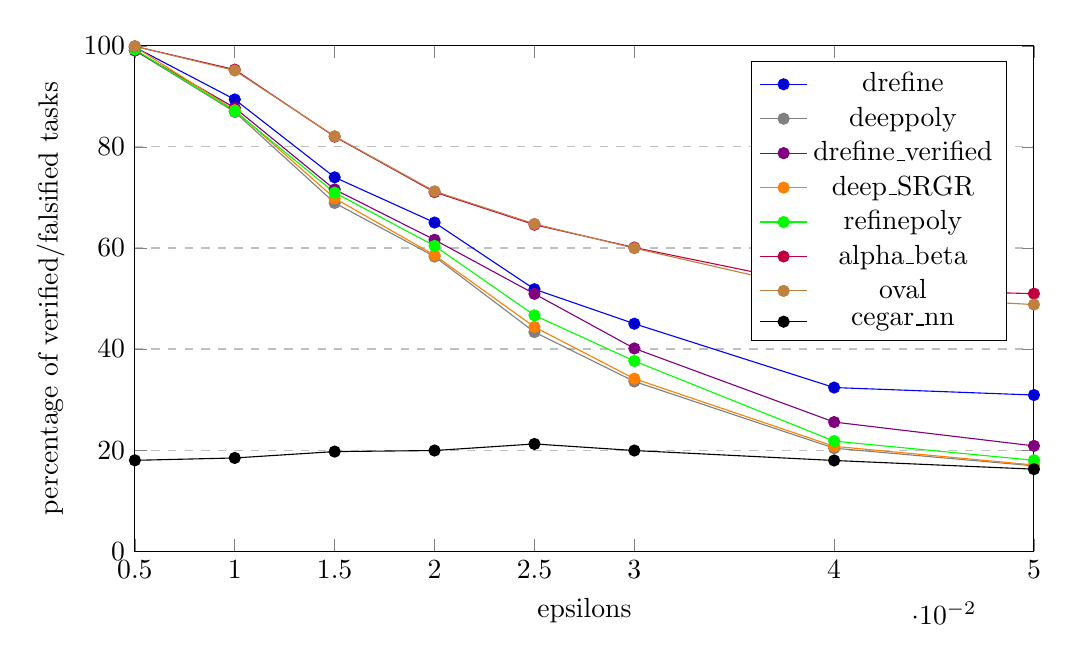
\begin{tikzpicture}
    \begin{axis}[
        xlabel={epsilons},
        ylabel={percentage of verified/falsified tasks},
        width=13cm,
        height=8cm,
        xmin=0.005, xmax=0.05,
        ymin=0, ymax=100,
        xtick={0.005,0.01,0.015,0.02,0.025,0.03,0.04,0.05},
        ytick={0,20,40,60,80,100},
        legend pos=north east,
        legend entries={drefine,deeppoly, drefine\_verified, deep\_SRGR, refinepoly, alpha\_beta, oval, cegar\_nn},
        ymajorgrids=true,
        grid style=dashed,
    ]
    \addplot+[
        color=blue,
        mark=*,
    ]
    coordinates {
        (0.005,99.72)(0.01,89.39)(0.015,73.98)(0.02,65.03)(0.025,51.84)(0.03,45.01)(0.04,32.38)(0.05,30.9)
    };

    \addplot[
        color=gray,
        mark=*,
    ]
    coordinates {
        (0.005,99.07)(0.01,86.9)(0.015,68.91)(0.02,58.3)(0.025,43.35)(0.03,33.58)(0.04,20.38)(0.05,16.89)
    };

    \addplot[
        color=violet,
        mark=*,
    ]
    coordinates {
        (0.005,99.07)(0.01,87.73)(0.015,71.58)(0.02,61.62)(0.025,50.92)(0.03,40.12)(0.04,25.55)(0.05,20.84)
    };

    \addplot[
        color=orange,
        mark=*,
    ]
    coordinates {
        (0.005,99.8)(0.01,87.26)(0.015,69.83)(0.02,58.57)(0.025,44.37)(0.03,34.13)(0.04,20.75)(0.05,17.06)
    };

    \addplot[
        color=green,
        mark=*,
    ]
    coordinates {
        (0.005,99.26)(0.01,87.08)(0.015,70.94)(0.02,60.42)(0.025,46.67)(0.03,37.63)(0.04,21.78)(0.05,17.99)
    };

    \addplot[
        color=purple,
        mark=*,
    ]
    coordinates {
        (0.005,99.9)(0.01,95.29)(0.015,82.02)(0.02,71.05)(0.025,64.60)(0.03,60.09)(0.04,51.98)(0.05,50.96)
    };

    \addplot[
        color=brown,
        mark=*,
    ]
    coordinates {
        (0.005,99.9)(0.01,95.11)(0.015,82.1)(0.02,71.21)(0.025,64.76)(0.03,59.96)(0.04,50.92)(0.05,48.8)
    };

    \addplot[
        color=black,
        mark=*,
    ]
    coordinates {
        (0.005,17.98)(0.01,18.45)(0.015,19.71)(0.02,19.92)(0.025,21.22)(0.03,19.92)(0.04,17.95)(0.05,16.23)
    };


    \end{axis}

\end{tikzpicture}
  }
    \caption{Size of input perturbation (epsilon) vs. percentage of solved instances}
    \label{res:ep:milp_with_milp}
\end{figure}


\paragraph{Comparison with adversarially trained networks: }
The networks considered for evaluation in this study are the ones corresponding to the 4st, 9th, and 10th 
rows of Table~\ref{tb:nndetail}. These networks have been trained using adversarial techniques, 
where adversarial examples were generated using standard methods such as PGD/DiffAI, and the network was subsequently 
trained on these adversarial examples to enhance its robustness. Table~\ref{tb:matrix1} presents a 
pairwise comparison of verifiers on these adversarially trained networks, 
encompassing a total of 2223 benchmark instances. 
Our approach demonstrates significant superiority over \deeppoly{}, \kpoly{}, and \deepsrgr{} in terms of 
performance on these benchmarks. While \alphabeta{} and \ovaltool{} outperform our approach by approximately 
135 benchmarks, we are still able to solve 75 unique benchmarks that remain unsolved by both of these tools. 
Considering the total number of benchmarks is 2223, this indicates a notable number of benchmarks that our 
approach successfully addresses.


{\color{red}
\begin{table}[t]
  \scriptsize
    \centering
    \begin{tabular}{|c|c|c|c|c|c|g||c|}
        \hline
        \diagbox{\tiny Verified}{\tiny \mbox{}\hspace{-2mm}Unverified} & \tiny \textbf{\deeppoly} & \tiny \textbf{\kpoly} & \tiny \textbf{\deepsrgr} & \tiny \textbf{\alphabeta} & \tiny \textbf{\ovaltool} & \tiny \textbf{\drefine} & \tiny \textbf{\textsc{total}} \\
        \hline
        \tiny \textbf{\deeppoly} & \textbf{0} & 0 & 0 & 3 & 3 & 0 & 1626 \\
        \hline
        \tiny \textbf{\kpoly} & 9 & \textbf{0} & 9 & 5 & 4 & 2 &  1635 \\ 
        \hline
        \tiny \textbf{\deepsrgr} & 2 & 2 & \textbf{0} & 3 & 3 & 0 & 1628 \\ 
        \hline
        \tiny \textbf{\alphabeta} & 302 & 295 & 302 & \textbf{0} & 1 & 205 & 1925 \\ 
        \hline
        \tiny \textbf{\ovaltool} & 312 & 304 & 310 & 11 & \textbf{0} & 214 & 1935 \\
        \hline
        \rowcolor{green!20}
        \tiny \textbf{\drefine} & 170 & 163 & 168 & 76 & 75 & \textbf{0} & 1796 \\
        \hline
    \end{tabular}
    % \caption{Pairwise comparison of tools on adversarially trained networks, e.g. entry on row \kpoly{} and column \deeppoly{} represents 9 benchmark instances on which \kpoly{} verified but \deeppoly{} fails. The green row highlights the number of solved benchmark instances by \drefine{} and not others while the red column is the opposite.}
    \caption{Pairwise comparison of tools on adversarially trained networks}
    \label{tb:matrix1}
\end{table}
}

% \paragraph{Number of marked neurons: }
% On average, \drefine{} marks $9.8\%$ of neurons, whenever it needs to refine. 
% Our experiments show that the number of marked neurons is quite small, so our refinement is indeed fast and strengthens the argument that {\em "finding causes of spuriousness"} does improve the overall efficiency. 

\paragraph{Detailed comparison with \alphabeta{} with same preprocessing: } 
To evaluate the effectiveness of our approach, we conducted a benchmark analysis on the instances where 
refinement was applied. We applied the same preprocessing steps used by \alphabeta{} to filter the benchmarks.

These include the so-called PGD (Projected Gradient Descent) attack, followed by CROWN~\cite{zhang2018efficient} which is an incomplete technique. The PGD attack is a method that can generate counter examples. It works by iteratively updating the  perturbation in the direction of the gradient of the loss function with respect to the input data,  while constraining the magnitude of the perturbation to be within a predefined limit. The CROWN technique generates the over-approximated bounds. %These preprocessing steps are PGD attack and CROWN. PGD attack is to generate the counter example and if it fails then CROWN runs to generate the bounds.

After preprocessing, the total number of benchmarks was reduced to $2362$, which were the benchmarks that were not 
solved by preprocessing steps. Out of these benchmarks, \alphabeta{} was able to verify $626$, 
while our approach verified 
$570$ benchmarks. Notably, our approach was able to solve $311$ benchmarks that were not solved by \alphabeta{}, 
while \alphabeta{} solved $366$ benchmarks that were not solved by our approach. 
\textit{All $311$ benchmarks solved by our approach were from adversarially trained networks, while 
not a single benchmarks out of $366$ solved by \alphabeta{} from adversarially trained networks}, 
suggesting that our approach performs 
well for such networks as PGD attack is not very effective on these benchmarks. 
These results indicate that the majority of the benchmarks ($1095$) solved by \alphabeta{} and not by our approach, 
as shown in Table~\ref{tb:matrix}, are likely solved by preprocessing steps rather than the refinement procedure.
The combination of benchmarks solved by both tools results in a total of 937 benchmarks, 
demonstrating an improvement in the benchmarks solved by \alphabeta{}. 
This highlights the significant contribution of our tool in the context of portfolio verifiers, 
as it complements and enhances the overall performance when integrated with other verification tools.


\paragraph{Subroutine time: }
% Table~\ref{tb:subroutine} presents the average time required by the \textsc{getmarkneuron} and \textsc{refinement} 
% subroutines, as well as the average number of marked neurons and refinement iterations in our experiments. 
% Each row in the table displays the average number for all benchmarks instances for a specific neural network. 
% The total average time taken by the \textsc{getmarkneuron} subroutine is $15.66$ seconds, while the \textsc{refinement}
% subroutine takes $89.69$ seconds. In comparison to the average \textsc{refinement} time, the \textsc{getmarkneuron} 
% subroutine takes up only $14.86\%$ of the total time, which is a small fraction. 
% The average number of marked neurons and refinement iterations are also relatively small, 
% indicating that integrating our \textsc{getmarkneuron} method with an efficient refinement procedure could significantly 
% improve overall performance. 


We conducted measurements to determine the average time required by the \textsc{getmarkneuron} subroutine 
and the \textsc{refinement} subroutine. 
The \textsc{getmarkneuron} subroutine exhibited an average execution time of $15.66$ seconds, 
whereas the \textsc{refinement} subroutine took $89.69$ seconds on average. 
Comparatively, the \textsc{getmarkneuron} subroutine accounted for only $14.86\%$ of the total time, 
which represents a small proportion. Furthermore, we measured the average number of marked neurons, 
which amounted to $14.81$, and the average refinement iteration count, which stood at $3.19$. 
These values also indicate a relatively small magnitude. 
These findings suggest that integrating our \textsc{getmarkneuron} method with an efficient refinement 
procedure could yield significant enhancements in overall performance.


% \begin{table}[t]
%   \centering
%   \scalebox{0.8}{
%   \begin{tabular}{c|c|c|c|c}
%           \hline
%           \textbf{Neural Network} & \textbf{Avg marking time} & \textbf{Avg refinement time} & \textbf{\#Mark Neurons} & \textbf{\#Refinement iterations} \\
%           \hline
%           $3\times 50$ & 0.39 & 112.50 & 22.17 & 4.63 \\
%           $3\times 100$ & 0.56 & 149.50 & 20.60 & 3.67  \\
%           $5\times 100$ & 1.97 & 6.10 & 5.23 & 1.5  \\
%           $6\times 100$ & 5.86 & 218.87 & 23.27 & 4.55 \\
%           $9\times 100$ & 66.90 & 109.32 & 38.1 & 8.80  \\
%           $6\times 200$ & 16.08 & 54.16 & 15.23 & 3  \\
%           $9\times 200$ & 42.32 & 58.72 & 11.17 & 2.17  \\
%           $6\times 500$ & 6.50 & 30.75 & 1.97 & 1.4  \\
%           $6\times 500$ & 7.5 & 133.20 & 5.45 & 1.2 \\
%           $4\times 1024$ & 8.56 & 23.80 & 5 & 1 \\
%           \hline
%           \textbf{Total average} & 15.66 & 89.69 & 14.81 & 3.19 \\
%           \hline
%       \end{tabular}
%       }
%       \caption{Avrage marking, refinement time and average number of marked neurons and refinement iterations}
%       \label{tb:subroutine}
%   \end{table}

% Figures \ref{res:milp_with_milp} and \ref{res:ep:milp_with_milp} shows that we are performing better in compare to
% the most related techniques \deeppoly{}, \texttt{refinepoly} and \texttt{deepSRGR}. 


% \todo{recall what is epsilon... x axis label can perhaps be written out more}



%--------------------- DO NOT ERASE BELOW THIS LINE --------------------------

%%% Local Variables:
%%% mode: latex
%%% TeX-master: "../main"
%%% End:

